\documentclass{book}
\usepackage{commeunjeustyle}
\begin{document}
%%%%%%%%%%%%%%%%%%%%%%%%%%%%%%%%%%%%%%%%%%%%%%%%%%%%%%%%%%%%%%%%%%%%%%
\chapter*{Série numérique}
%%%%%%%%%%%%%%%%%%%%%%%%%%%%%%%%%%%%%%%%%%%%%%%%%%%%%%%%%%%%%%%%%%%%%%

En mathématiques, la notion de série permet de généraliser la notion de somme finie.\\
\'Etant donnée une suite  $(u_n)_{n\in\N}$, étudier la série de terme général $u_n$ c'est étudier la suite $(S_n)_{n\in\N}$ obtenue en prenant la somme des premiers termes de la suite $(u_n)_{n\in\N}$, c'est à dire :
$$ S_{n}=u_{0}+u_{1}+\cdots +u_{n}=\sum _{k=0}^{n}u_{k}.$$
Peut-on donner un sens à la somme de tous les termes d'une suite infinie de nombres
réels : 
$$
\lim_{n\to\infty}S_n= u_{0}+u_{1}+u_{3}+u_{4}+\cdots =\lim_{n\to\infty}\sum _{k=0}^{n}u_{n} ?$$ 
Peut-on  permuter les termes de la suite ou opérer des regroupement sans modifier ni la convergence ni la somme de la série ?
\begin{Exemple}[Partager un carré]
Peut-on partager un carré en une infinité de
rectangles de façon à enlever à chaque étape la moitié de l'aire restante ? La figure ci-dessous montre une solution.
\begin{center}
 \begin{picture}(128,128)
\put(0,0){\line(1,0){128}}
\put(0,0){\line(0,1){128}}
\put(128,0){\line(0,1){128}}
\put(0,128){\line(1,0){128}}
\put(96,64){\text{$\frac{1}{2}$}}
\put(64,0){\line(0,1){128}}
\put(32,96){\text{$\frac{1}{4}$}}
\put(0,64){\line(1,0){64}}
\put(48,32){\text{$\frac{1}{8}$}}
\put(32,0){\line(0,1){64}}
\put(16,48){\text{$\frac{1}{16}$}}
\put(0,32){\line(1,0){32}}
\put(18,10){\text{$\frac{1}{32}$}}
\put(16,0){\line(0,1){32}}
\put(0,16){\line(1,0){16}}
\put(8,0){\line(0,1){16}}
%\put(0,16){\line(0,1){32}}
\end{picture}
\end{center}
En prenant comme unité d'aire, l'aire du carré de départ, on en déduit la relation :
$$ 1 =\frac{1}{2}+ \frac{1}{4}+\frac{1}{8}+\frac{1}{16}+\frac{1}{32}+\dots= \lim_{n\to\infty}\sum_{k=1}^n 2^{-k}.$$ 
La somme de tous les termes de la suite $(2^{-n})_{n\in\N^*}$ converge et est égale à 1.
\end{Exemple}
\begin{Exemple}[Somme harmonique]
La somme harmonique est la somme des inverses des entiers naturels non nuls qui est donc égale à
$$ H_{n}=1+{\frac {1}{2}}+{\frac {1}{3}}+{\frac {1}{4}}+\cdots +{\frac {1}{n}}=\sum _{k=1}^{n}{\frac {1}{k}}.$$
On peut remarquer\footnote{On peut aussi regrouper les termes 
$$ \lim_{n\to\infty}H_{n}=1+{\frac {1}{2}}+\overbrace{\frac {1}{3}+\frac {1}{4}}^{\geq \frac 1 2}_{2 \text{ termes}}+\overbrace{\frac {1}{5}+\frac {1}{6}+\frac {1}{7}+\frac {1}{8}}^{\geq \frac 1 2}_{4 \text{ termes}}+\overbrace{\frac {1}{9}+\dots+\frac {1}{16}}^{\geq \frac 1 2}_{8 \text{ termes}}+\dots$$
et la limite est donc supérieur à une somme infini de $1/2$ donc la limite est l'infinie (voir \url{https://www.youtube.com/watch?v=_AtkIpi6KP0}).} que l'aire sous la courbe rouge est inférieur à la somme des aires des rectangles oranges 
\begin{center}
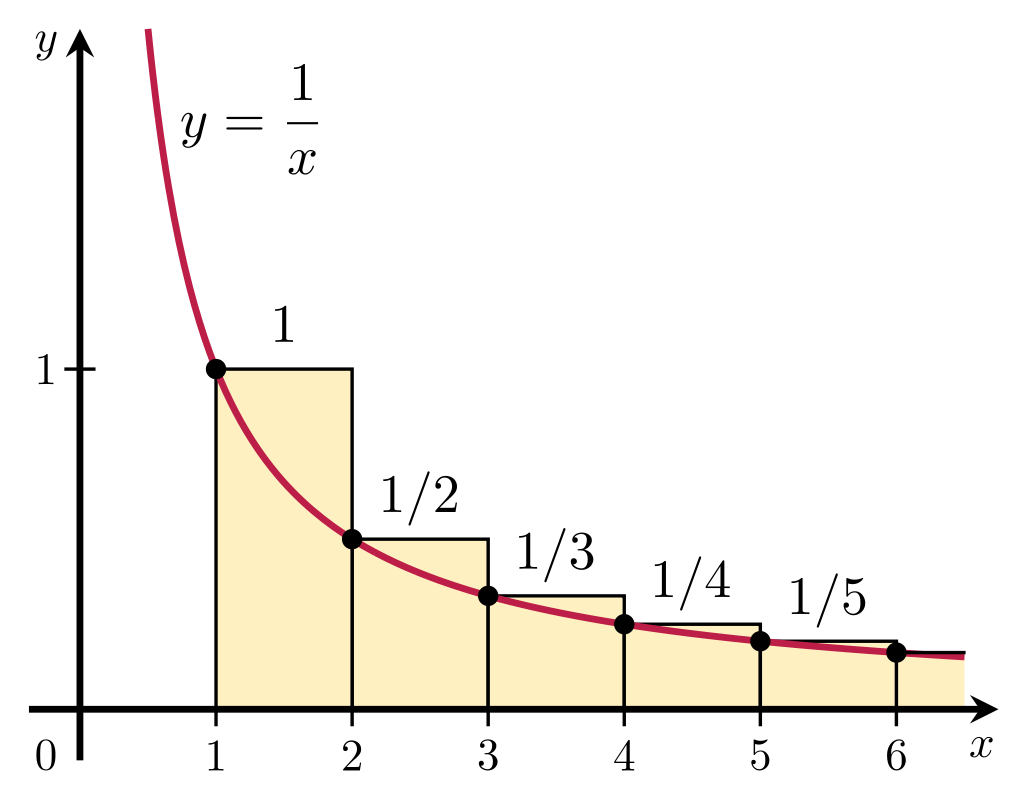
\includegraphics[width=6cm]{serie_numerique_fig_serie_harmonique}
\end{center}
d'où
$$ H_{n}=1+{\frac {1}{2}}+{\frac {1}{3}}+{\frac {1}{4}}+\cdots +{\frac {1}{n}}\geq\int_1^{n+1}\frac 1 x dx=\ln(n+1).$$
Comme  $\lim\limits_{n\to\infty}\ln(n+1)=+\infty$, la suite $(H_n)$ diverge.\\
La somme de tous les termes de la suite $(1/n)_{n\in\N}$ diverge vers l'infini.
\end{Exemple}
\begin{Exemple}[Non commutativité des sommes infinies]
On considère cette somme
$$ S_{n}=1-{\frac {1}{2}}+{\frac {1}{3}}-{\frac {1}{4}}+\cdots +{\frac {(-1)^{n+1}}{n}}.$$
On a $$\lim_{n\to\infty}S_{n}=\overbrace{1-{\frac {1}{2}}}^{\geq \frac 1 2}+\overbrace{\frac {1}{3}-\frac {1}{4}}^{\geq  0}+\overbrace{\frac {1}{5}-\frac {1}{6}}^{\geq  0}+\cdots \geq \frac 1 2.$$
En réorganisant les termes, on obtient :
	$$\begin{aligned}
	\lim_{n\to\infty}S_{n}&= \left(1 - \frac 1 2\right) - \frac 1 4 + \left(\frac 1 3 - \frac 1 6\right)- \frac 1  8+ \left(\frac 1 5 - \frac{1}{10}\right)\cdots  \\
					     &=\frac 1 2 - \frac 1 4  + \frac 1 6 - \frac 1  8+  \frac{1}{10}+ \cdots\\
					     &=\frac 1 2 (1-{\frac {1}{2}}+{\frac {1}{3}}-{\frac {1}{4}}+{\frac {1}{5}}+\cdots)\\
					     &=\frac 1 2 (\lim_{n\to\infty}S_{n})\\
					     &=0
	\end{aligned}$$
D'où une contradiction car $\lim_{n\to\infty}S_{n}\geq \frac 1 2 $ et $\lim_{n\to\infty}S_{n}=0$.
\end{Exemple}
\newpage

\section{Généralités}


\begin{Definition}[Série numérique]
Soit $(u_n)_{n\in\N}$ une suite numérique.\\
On appelle suite des \defi{somme partielle} donnée par pour tout $n\in\N$, $S_n=u_0+u_1+\dots+u_n=\sum _{k=0}^{n}u_{k}$.\\
La suite   $(S_n)_{n\in\N}$ est appelée \defi{série numérique} de \defi{terme général} et noté $\sum u_n$.
\end{Definition}
\begin{Exemple}
La somme partielle de  la série harmonique $\sum \frac 1 n$ est  égale à $S_n=1+\frac 1 2 +\frac 1 3+\cdots +\frac 1 n$. 
\end{Exemple}
\begin{Definition}
On dit que la série $\sum u_n$ est convergente (respectivement divergente, majorée, minorée, bornée, croissante ou décroissante) si et seulement si la suite $(S_n)_{n\in\N}$ l'est.\\
Dans ce cas, on appelle \defi{somme de la série} la limite $S$ de la suite de ses sommes partielles $(S_n)_{n\in\N}$, et on la note $\sum_{n=0}^{+\infty} u_n$.
Ainsi, 
\begin{center}
\shadowbox{
$S = \sum_{n=0}^{+\infty} u_n = \lim_{n\to\infty} S_n = \lim_{n\to\infty} \sum_{k=0}^n u_k.$
}
\end{center}
De plus, on appelle \defi{reste} d'ordre $n$ de la série la quantité
\begin{center}
\shadowbox{
$R_n = S - S_n = \sum_{k=0}^{+\infty} u_k -\sum_{k=0}^n u_k = \sum_{k=n+1}^{+\infty} u_k = \sum_{k>n} u_k.$
}
\end{center}
On a :
$$ \lim_{n\to\infty}R_n=0.$$
\end{Definition}


\begin{Remarque} Attention :
\begin{itemize}
\item $\sum u_n$ est une suite,
\item $\sum_{k=0}^n u_k$ est un nombre,
\item $\sum_{n=0}^\infty u_n$ est un nombre si la série est convergente.
\end{itemize}
\end{Remarque}

\begin{Exemple}[Série géométrique]
Soit $\sum q^n$ la série géométrique.
Pour $q\ne 1$, on a :
$$\begin{aligned}
	S_{n}&= 1+q+q^2+\dots+q^n  \\
	-qS_{n}&=-q-q^2+\dots+q^n-q^{n+1} \\
	S_{n}-qS_{n}&= 1 -q^{n+1}
\end{aligned}$$
$$ S_{n} = \frac{1-q^{n+1}}{1-q} $$
La série converge  si et seulement si $|q|<1$. Dans le cas de convergence,  sa somme est $\frac{1}{1-q}$. \\
On retrouve par exemple que $\frac 1 9= 0,111\dots$, d'où $1 = 0, 999\dots$ car $0,111\dots=\sum_{n=1}^{\infty}\left(\frac{1}{10}\right)^n=\frac{1/10}{1-1/10}=\frac{1}{9}.$

\end{Exemple}

\begin{Exemple}[Séries télescopiques]
Soit $(a_n)_{n\in\N}$ une suite numérique et $u_n = a_{n+1} - a_n$.\\
On a $$\begin{aligned}
S_n &= (a_1 - a_0)+ (a_2 - a_1)+\cdots+(a_{n+1} - a_n)\\&=a_{n+1}-a_0.\end{aligned}$$
Donc la série $\sum u_n$ télescopiques converge si et seulement si la suite $(a_n)_{n\in\N}$ converge. Si la série converge, sa limite est  $\lim\limits_{n\to\infty}a_n-a_0$.\\
Par exemple, la série $\sum \frac{1}{n(n+1)}=\sum\left(\frac{1}{n}-\frac{1}{n+1}\right)$ converge vers $1$. 
\end{Exemple}

\begin{Proposition}[Indépendance du rang]
Pour tout $ n_0 \in \N$, les séries $\sum_{n\geq 0}u_n$ et  $\sum_{n\geq n_0}u_n$ sont de même nature,
c'est-à-dire ou toutes deux convergentes ou toutes deux divergent.
\end{Proposition}
\begin{Demonstration}
$$\begin{aligned}
\sum_{n\geq 0}u_n \text{ converge}\Leftrightarrow &\forall \epsilon \in \R^{+*}, \exists N\in N, \forall n \geq N:  |\sum_{k=0}^{n}u_k-\sum_{k=0}^{\infty} u_k|\leq \epsilon\\
\Leftrightarrow &\forall \epsilon \in \R^{+*}, \exists N\in N, \forall n \geq N:  |\sum_{k=n_0}^{n}u_k-(\sum_{k=0}^{\infty} u_k-\sum_{k=0}^{n_0-1}u_k)|\leq \epsilon\\
\Leftrightarrow &\sum_{n\geq n_0}u_n \text{ converge.}
\end{aligned}$$  
\end{Demonstration}




\begin{Proposition}[Espace vectoriel]
L'ensemble des séries convergentes est un espace vectoriel, c'est à dire si $\sum u_n$ et $\sum v_n$ convergent vers $S$ et $S'$, la série $\sum (a u_n + b v_n)$ converge pour toutes constantes réelle $a,b$. De plus, dans ce cas, le somme est  $aS+bS'$.
\end{Proposition}
\begin{Demonstration}
Voir le cours sur les suites. 
\end{Demonstration}
\begin{Exemple}
La série $\sum \left(3 (\frac{\sqrt{2}}{2})^n-5(0.999)^n\right)$ converge.
\end{Exemple}
\begin{Remarque} Attention la réciproque est FAUSSE ($\sum (a u_n + b v_n)$ converge implique que $\sum u_n$ et $\sum v_n$ convergent).
Comme contre-exemple, la série $\sum \frac{1}{n(n+1)}=\sum \left(\frac{1}{n}-\frac{1}{n+1}\right)$ est convergente comme série télescopique. Cependant la série harmonique $\sum \frac{1}{n}$ est divergente.  
\end{Remarque}






\begin{Proposition}[Grossièrement divergente]
Soit $\sum u_n$ une série numérique.\\
Si la série converge, alors $ \lim_{n\to\infty}u_n= 0$.\\
On dit que la série numérique $\sum u_n$ est \defi{grossièrement divergente} si $u_n$ ne tend pas vers 0.
\end{Proposition}
\begin{Demonstration}
Soit $\sum u_n$ une série convergente.
On a $u_n = S_{n}-S_{n-1}.$ Par passage à la limite (l'ensemble des suites convergentes est un espace vectoriel), on a  :$$\lim_{n\to\infty}u_n =\lim_{n\to\infty}( S_{n}-S_{n-1})=S-S=0.$$
\end{Demonstration}
\begin{Remarque}
La réciproque est fausse.
Le contre-exemple classique est la série harmonique
$\sum_{n\geq 1} \frac1n$ qui est divergente,
bien que $ \lim_{n\to\infty} \frac1n =0$.
\end{Remarque}
%
%
%%% -----------------------------------------------------------------------------
\section{Séries à termes positifs (SATP)}

\subsection{Croissance des sommes partielles}
%\begin{intr}
Les séries à termes positifs jouent un rôle clé dans la théorie des séries. Si elle diverge, alors la suite des sommes partielles tend vers $+\infty$. Les
possibilités de divergence sont bien plus diverses pour une série dont les termes changent de signe une infinité de fois.

Pour comprendre le comportement d'une série $\sum u_n$ à termes positifs, il convient d'observer que dans ce cas la suite de ses sommes partielles $(S_n)$ est une suite croissante de réels positifs. En effet, pour tout $n \geq 1 , S_n - S_{n-1}= u_n \geq  0$, donc $S_n \geq S_{n-1}$. Il est commode de représenter une telle suite croissante $(S_n)$ par un escalier infini, où la $n^e$ marche est
le segment horizontal d'extrémités les points de coordonnées $(n, S_n)$ et $(n+1, S_n)$. Ainsi la figure 1.2 représente  l'escalier associé à la série harmonique
(en posant $u_0 = 0)$,
\begin{figure}[!h]
\begin{center}
\begin{tikzpicture}
\draw[red,very thick] (0,0) -- (1,0) -- (1,1) -- (2,1) -- (2,1.5) -- (3,1.5) -- (3,1.83) -- (4,1.83) -- (4,2.08) -- (5,2.08) -- (5,2.28) -- (6,2.28) -- (6,2.44) -- (7,2.44) -- (7,2.59) -- (8,2.59);
\draw[thick,->] (0,0) -- (8.5,0) node[anchor=north west] {$x$};
\draw[thick,->] (0,0) -- (0,3.5) node[anchor=south east] {$y$};
\foreach \x in {0,1,2,3,4,5,6,7,8}
   \draw (\x cm,1pt) -- (\x cm,-1pt) node[anchor=north] {$\x$};
\foreach \y in {0,1,2,3}
    \draw (1pt,\y cm) -- (-1pt,\y cm) node[anchor=east] {$\y$};
\end{tikzpicture}
\caption{Escalier infini de la série harmonique}
\end{center}
\end{figure}


Sur cette figure, on voit que la pente est de plus en plus douce, mais comme dans le cas
d'une représentation graphique de fonction, cela ne suffit pas pour conclure à l'existence
d'une asymptote horizontale. On observe le même phénomène avec la représentation graphique de la fonction logarithme et il est bien connu que $\ln x$ tend vers l'infini quand $x$
tend vers l'infini et donc qu'il ne peut y avoir d'asymptote horizontale.


Pour un escalier infini représentant une série à termes positifs, il y a que deux  possibilités :
\begin{itemize}
\item ou bien l'escalier est plafonné, autrement dit il existe une altitude $M$
qu'il ne peut jamais franchir (mathématiquement, $M$ est un majorant de l'ensemble
de toutes les valeurs de la suite $(S_n)_{n\in\N}:  \forall n \in \N, S_n \leq M)$ ;
\item ou bien il n'est pas plafonné et finit donc par dépasser toute altitude fixée à l'avance.
Dans le deuxième cas, comme la suite $(S_n)_{n\in\N}$ est croissante, pour chaque altitude $A$
fixée, à partir d'un certain rang $n_0$, $S_{n}\geq A$ pour tous les indices suivants.
Comme A est quelconque, cela signifie que $(S_n)_{n\in\N}$ tend vers l'infini.
\end{itemize}
%\end{intr}


\begin{Definition}[Série à termes positifs]
Une \defi{série à termes positifs} est une série réelle $\sum u_n$ telle que $$\forall n\in\N,\quad u_n\geq 0.$$
\end{Definition}
\begin{Proposition}[Adaptation du théorème de la limite monotone]
Une SATP converge si et seulement si la suite de ses sommes partielles est majorée.\\
De plus, si elle converge, sa somme est égale à la borne supérieure
des sommes partielles.\\
De plus, si elle diverge, elle diverge vers l'infinie. 
\end{Proposition}
\begin{Demonstration}
Comme $S_{n+1}-S_n=u_{n+1}\geq 0$, la suite $(S_n)_{n\in\N}$ est croissante. Une suite croissante converge si set seulement si la suite est majorée. De plus, si elle converge, sa somme est égale à la borne supérieure.
\end{Demonstration}

\subsection{Règles de convergence}


\begin{Proposition}[Règle de comparaison]
\label{prop:satp}
Soit $(u_n)_{n\in\N}$ et $(u_n)_{n\in\N}$ deux suites réelles tel que $$\forall n\in\N,\quad 0\leq u_n\leq v_n.$$
\begin{itemize}
\item
  Si $\sum v_n$ converge, alors $\sum u_n$ converge également.
\item
  Si $\sum u_n$ diverge, alors $\sum v_n$ diverge également.
\end{itemize}
\end{Proposition}
\begin{Demonstration}
Soit $(u_n)_{n\in\N}$ et $(u_n)_{n\in\N}$ deux suites réelles tel que $\forall n\in\N,\quad 0\leq u_n\leq v_n.$
Soit  $\sum v_n$ convergente. 
$\sum u_n$ est une SATP.  On a : 
$$\forall n \in \N : \quad \sum_{k=0}^n u_n\leq  \sum_{k=0}^n v_n \overbrace{\leq}^{\text{théorème de limité monotome}}  \sum_{k=0}^{+\infty} v_n<+\infty.$$
Comme la suite des sommes partielles est bornée, d'après la proposition précédente,  $\sum u_n$ est convergente. Idem pour la divergence.
\end{Demonstration}

\begin{Remarque}
Les inégalités $$\quad 0\leq u_n\leq v_n$$  peuvent être vérifiées uniquement à partir d'un certain rang car la convergence ou la divergence d'une série ne dépendent pas des premiers termes. 
\end{Remarque}
\begin{Exemple}
Étudions la nature de la  série $\sum e^{-n^2}$ à termes positifs. On a  $\forall n\in\N : 0\leq e^{-n^2}\leq e^{-n}=(\frac 1 e)^n$. Comme la série géométrique $\sum \left(\frac 1 e\right)^n$ est convergente car $|\left(\frac 1 e\right)|<1$, la série $\sum e^{-n^2}$ est convergente d'après la règle de comparaison. 
\end{Exemple}

\begin{Proposition}[Règle du petit o et grand O] \label{prop:comp}
Soit $\sum u_n$ et $\sum v_n$ deux SATP.
On suppose que $u_n = \GrandO_\ninf(v_n)$ (ou  $u_n = \PetitO_\ninf(v_n)$).
Alors:
\begin{itemize}
\item
  Si $\sum v_n$ converge, alors $\sum u_n$ converge également.
\item
  Si $\sum u_n$ diverge, alors $\sum v_n$ diverge également.
\end{itemize}
\end{Proposition} 
\begin{Demonstration}
On suppose $\sum v_n$ converge.\\
On a  $(u_n)$ et $(u_n)$ deux suites réelles positives tel que $u_n = \GrandO_\ninf(v_n)$. Cela signifie qu'il existe 
$ M\in \R^+,\forall n\geq N :\quad  u_n\leq M v_n.$\\
On a :
$$\forall n \in \N :	\sum_{k=0}^n u_k\leq \sum_{k=0}^n(M v_k) \leq M\sum_{k=0}^n v_k\overbrace{\leq}^{\text{théorème de limité monotome}} M\sum_{k=0}^{\infty} v_k $$
Donc la suite des sommes partielles est bornée, donc la série $\sum u_n$ est convergente. 
\end{Demonstration}
\begin{Exemple}
Étudions la nature de la  série $\sum \frac{1}{\sqrt{n}}$ à termes positifs. On a  $\frac{1}{n}=\PetitO_\ninf(\frac{1}{\sqrt{n}})$. Comme la série harmonique $\sum \frac 1 n$ est divergente, la série $\sum \frac{1}{\sqrt{n}}$ est divergente d'après la règle de comparaison. 
\end{Exemple}
\begin{Proposition}[Règle d'équivalence]
Soit $\sum u_n$ et $\sum v_n$ deux SATP telles que $u_n \Sim_\ninf v_n$.\\
Alors $\sum u_n$ et $\sum v_n$ sont de même nature.
\end{Proposition}
\begin{Demonstration}
$u_n \Sim_\ninf v_n$ implique que $u_n= \GrandO_\ninf(v_n)$ et que $v_n= \GrandO_\ninf(u_n)$. On conclut à l'aide de la proposition~\ref{prop:comp}.
\end{Demonstration}
\begin{Exemple}
Étudions la nature de la  série $\sum \frac{1}{\ln(1+n)}$ à termes positifs. On a  $\frac{1}{\ln(1+n)}\Sim_\ninf \frac 1 n$. Comme la série harmonique $\sum \frac 1 n$ est divergente,   la série $\sum \frac{1}{\ln(1+n)}$ est divergente d'après la règle d'équivalence. 
\end{Exemple} 

\begin{Proposition}[Règle de d'Alembert]
Soit une SATP $\sum u_n$.  On suppose que la suite $\left(\frac{u_{n+1}}{u_n}\right)_{n\in\N}$  est définie à partir d'un certain rang et admet une limite $L$  quand  $n$ tend vers $+\infty$.\\
Alors
\begin{itemize}
\item si $L<1$, la série $\sum u_n$ est convergente,
\item si $L>1$, la série $\sum u_n$ est divergente.
\end{itemize}
\end{Proposition}
\begin{Remarque}
Si $L=1$, on ne pas conclure. En effet, on a $L=1$ pour la série $\sum \frac{1}{n}$ et $\sum \frac{1}{n^2}$ et pourtant la première diverge et la seconde converge.   
\end{Remarque}

\begin{Demonstration}
Supposons   $L<1$. Soit $L\leq A\leq 1$.  A partir d'un certain rang $n_0$,  on a 
$$\forall  n\geq n_0 :\quad \frac{u_{n+1}}{u_n}\leq A$$
$$\forall  n\geq n_0 :\quad u_n \leq A^{n-n_0}u_{n_0}$$ 
La série géométrique $\sum_{n\geq n_0}  A^{n-n_0}$ converge car $|A|<1$. Par règle de comparaison, $\sum_{n\geq n_0}  u_n$ converge, donc $\sum  u_n$  convergente.\\
Supposons   $L>1$. Soit $L\geq A \geq 1$.  A partir d'un certain rang $n_0$,  on a 
$$\forall  n\geq n_0 :\quad \frac{u_{n+1}}{u_n}\geq A$$
$$\forall  n\geq n_0 :\quad u_n \geq A^{n-n_0}u_{n_0}$$ 
La série géométrique $\sum_{n\geq n_0}  A^{n-n_0}$  diverge car $|A|>1$. Par règle de comparaison, $\sum_{n\geq n_0}  u_n$ diverge, donc $\sum  u_n$ est diverge.
\end{Demonstration}
\begin{Exemple}[Série exponentielle]
Soit $a\in \R^+$. La série $\sum \frac{a^n}{n!}$ converge car d'après la règle de d'Alembert, on a :
$$\frac{ \frac{a^{n+1}}{(n+1)!}}{\frac{a^{n}}{(n)!}}=\frac{a}{n+1}\xrightarrow[n \to +\infty]{}0.$$
Dans le chapitre sur les séries entières, on définira la fonction exponentielle ainsi  $$\exp:x\to \sum_{n=0}^{+\infty} \frac{x^n}{n!}.$$
\end{Exemple}



%
%
%
\subsection{Comparaison série-intégrale}
Les séries sont un procédé de sommation de grandeurs discrètes, l'intégrale de grandeurs continues. L'analogie formelle entre les deux domaines permet de faire passer des idées intéressantes de l'une à l'autre. On compare ces deux objets mathématiques à l'aide d'inégalités.\\
\begin{tikzpicture}[scale=0.75]
\tkzInit[xmax=8,ymax=2]
\tkzAxeXY
\tkzGrid
\draw (1,1.3) node[above]{$x\to\frac 1 x $} ; 
\draw [domain=1:8,samples=200,color=red] plot (\x,{1/\x});  
\tkzFct[color = black]{1./(x)}
\tkzDrawRiemannSumSup[fill=green!60,
                     opacity=.2,
                     color=green,
                     line width=1pt,
                     interval=1:8,
                     number=7] 
\foreach \x/\t in {1.5/$1$,2.5/$\frac12$,3.5/$\frac13$}
\node[green!50!black] at (\x,{(1/(\x-0.5))+0.2}){\t}; 
\end{tikzpicture}
\begin{tikzpicture}[scale=0.75]
\tkzInit[xmax=8,ymax=2]
\tkzAxeXY
\tkzGrid
\draw (1,1.3) node[above]{$x\to\frac 1 x $} ; 
\draw [domain=1:8,samples=200,color=red] plot (\x,{1/\x});  
\tkzFct[color = black]{1./(x)}
\tkzDrawRiemannSumInf[fill=blue!60,
                     opacity=.2,
                     color=blue,
                     line width=1pt,
                     interval=1:8,
                     number=7] 
\foreach \x/\t in {1.5/$\frac12$,2.5/$\frac13$,3.5/$\frac14$}
\node[blue!50!black] at (\x,{(1/(\x+0.5))+0.2}){\t}; 
\end{tikzpicture} \\
L'aire entre $1$ et $n$ est:
\begin{itemize}
\item sous la courbe rouge   : $\int_1^N f(x)dx$,
\item des rectangles verte  : $\sum_{n=1}^{N-1}f(n)$,
\item  des rectangles bleues  : $\sum_{n=2}^{N}f(n)$.
\end{itemize}
Géométriquement, on a les inégalités :
$$\sum_{n=1}^{N-1}f(n)\leq \int_1^N f(x)dx \leq \sum_{n=2}^{N}f(n).$$
Par passage à la limite, on a :
$$\sum_{n=1}^{+\infty}f(n)\leq \int_1^{+\infty} f(x)dx \leq \sum_{n=2}^{+\infty}f(n).$$
On peut affirmer que série $\sum f(n)$ converge si et seulement si la suite $\left( \int_1^n f(x) dx \right)_{n\in\N}$ converge.


\begin{Theoreme}[Comparaison série-intégrale]
Soit f continue sur $[1,+\infty[$, décroissante
et positive sur cet intervalle. \\
La série $\sum_{n\geq 1} f(n)$ converge si et seulement si la suite $\left( \int_{1}^n f(x) dx \right)_{n\in\N}$ converge.
\end{Theoreme}
\begin{Demonstration}
Par décroissance de $f$, on a :
$$\forall n> 0,\quad \forall x\in [n,n+1]:\quad f(n+1)\leq f(x) \leq f(n)$$
On intègre : 
$$\forall n> 0 : \quad \int_n^{n+1}f(n+1)dx\leq \int_n^{n+1}f(x)\,dx \leq \int_n^{n+1}f(n)dx$$
$$\forall n>0 : \quad f(n+1)\int_n^{n+1}dx\leq \int_n^{n+1}f(x)\,dx \leq f(n)\int_n^{n}dx$$
$$\forall n> 0 : \quad f(n+1)\leq \int_n^{n+1}f(x)\,dx \leq f(n)$$
En sommant ces inégalités depuis $1$ jusqu'à $N-1$, les intégrales se raccordent et l'on obtient : 
 $$\sum_{n=2}^{N}f(n)\leq \int_1^N f(x)\,dx \leq \sum_{n=1}^{N-1}f(n).$$
Supposons que la série $\sum_{n\geq 1} f(n)$ converge. Comme $\int_1^N f(x)dx \leq \sum_{n=1}^{N-1}f(n)<+\infty$, la suite croissante $\left( \int_{1}^n f(x)\, dx \right)_{n\in\N}$ est  bornée donc convergente. \\
Supposons que la série $\sum_{n\geq 1}f(n)$ diverge. Comme elle est à termes positifs, elle diverge vers l'infini.  Comme $\sum_{n=2}^{N}f(n)\leq \int_1^N\, f(x)dx$, la suite croissante $\left( \int_{n_0}^n f(x) dx \right)_{n\in\N}$ n'est pas bornée donc divergente. 
\end{Demonstration}
\begin{Theoreme}[Comparaison série-intégrale (version intégrale impropre)]
Soit f continue sur $[1,+\infty[$, décroissante
et positive sur cet intervalle. \\
La série $\sum_{n\geq 1} f(n)$ et l'intégrale $\int_{1}^\infty f(x) dx$ sont de même nature.
\end{Theoreme}
\begin{Proposition}[Séries de Riemann]
La série $\sum \frac{1}{n^a}$ converge si et seulement si $a> 1$.
\end{Proposition}
\begin{Demonstration}
Pour $a\leq 0$, le terme général de la série ne tend pas vers 0 en l'infini donc la série diverge grossièrement.\\
Pour $a>0$, on applique le théorème de la comparaison série-intégrale avec la fonction $f:x\to\frac{1}{x^a}$ décroissante et continue sur $[1,+\infty[$.\\
De plus si $a\neq 1$, on a   :
$$ \int_{1}^n \frac{1}{x^a} dx =
\left[\frac{1}{(-a+1)x^{a-1} }\right]_1^n=\frac{1}{-a+1}\left(\frac{1}{n^{a-1}}-1\right) \xrightarrow[n\to \infty]{}\begin{cases}
\frac{1}{a-1} \text{ si }a> 1 \\
+\infty\text{ si }a< 1
\end{cases}.$$ 
De plus si $a= 1$, on a   :
$$ \int_{1}^n \frac{1}{x} dx = \ln n  \xrightarrow[n\to \infty]{}+\infty .$$ 
En conclusion, la série $\sum \frac{1}{n^a}$ converge si et seulement si $a> 1$.
%$$ \int_{1}^n f(x) dx =\begin{cases}
%\left[\frac{1}{(-a+1)x^{a-1} }\right]_1^n=\frac{1}{-a+1}\left(\frac{1}{n^{a-1}}-1\right) \text{ si }a\neq 1 \t\\
%\left[\ln x\right]_1^n=\ln n  \text{ si }a=1
%\end{cases}$$ 
\end{Demonstration}

\section{Séries à termes de signe variable}
\subsection{Absolument convergente}
Nous passons maintenant à l'étude des séries qui ne sont pas à termes positifs. Pour expliquer le titre de cette section,
 il convient de remarquer que si le signe de $u_n$ est constant
à partir d'un certain rang $n_0$, l'étude de la convergence de $\sum u_n$ se ramène à celle d'une
série à termes positifs. En effet, $\sum_{n\geq 0} u_n$et $\sum_{n\geq n_0} u_n$ sont de même nature et si $u_n < 0$ à partir du rang $n_0$, il suffit de considérer la série $\sum
_{n\geq n_0} (-u_)n$.

Ce que nous allons voir dans cette section n'est donc réellement nouveau que pour les séries dont le terme général change de signe
une infinité de fois.

Une première idée pour l'étude des séries à terme de signe variable est d'exprimer ses
sommes partielles comme différences de sommes partielles de deux séries à termes positifs.
Pour cela, il suffit d'utiliser la décomposition $u_n = u_n^+-u_n^-$ où $u_n^+$ est la partie positive
du réel $u_n$ et $u_n^-$
sa partie négative\footnote{Soit $x$ un nombre réel. Sa
partie positive $x^+$
 et sa partie négative $x^-$ sont les réels positifs :
$$x^+=\max(0,x), \quad x^-=\max(0,-x).$$
On a les égalités suivantes : 
$$x=x^+-x^-,\quad |x|=x^++x^-,\quad x^+=\frac{x+|x|}{2}\quad x^-=\frac{-x+|x|}{2}$$
et les inégalités suivantes :
$$0\leq x^+ \leq |x| , \quad 0\leq x^- \leq |x|.$$
}.
On a :
$ \sum_{k=0}^n u_k= \sum_{k=0}^n (u^+_k-u^-_k) = \sum_{k=0}^n u_k^+ -  \sum_{k=0}^n u_k^-.$
Une condition suffisante pour que la série $\sum u_n$ converge et que les deux SATP $\sum u_k^+$ et $\sum u_k^-$ convergent. 
Compte tenu des inégalités $0\leq u_n^+ \leq |u_n| , \quad 0\leq u_n^- \leq |u_n|$, le
théorème de comparaison des séries à termes positifs nous permet de conclure qu'une
condition suffisante pour la convergence de $\sum u_k^+$ et $\sum u_k^-$
et donc aussi $\sum|u_n|$ converge. Nous venons ainsi d'établir le résultat le plus important pour
la convergence d'une série à termes de signe variable.\\
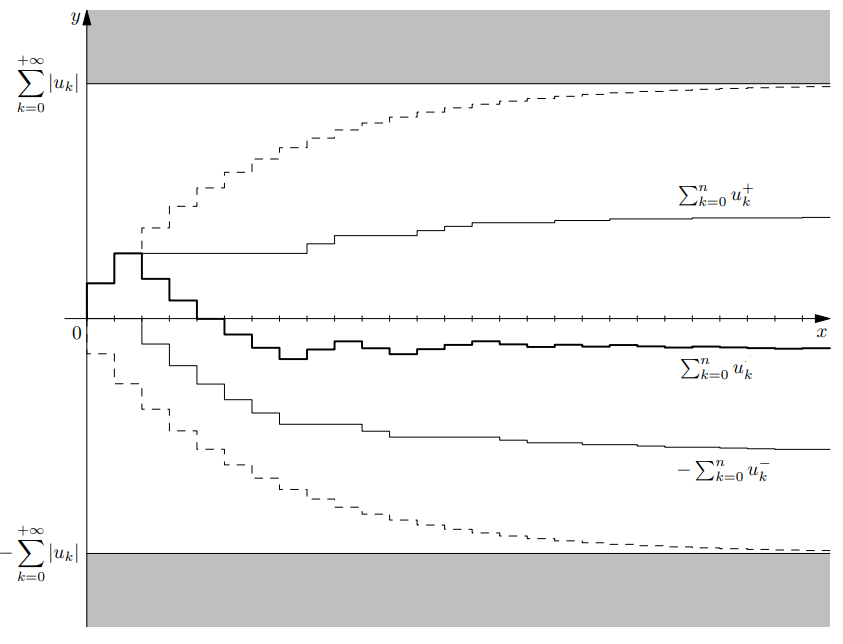
\includegraphics[scale=0.8]{serie_numerique_fig_1.png}

\begin{Theoreme}
Si la SATP $\sum |u_n|$ converge alors $\sum u_n$ converge.
\end{Theoreme}
\begin{Definition}[Absolue convergence]
La série est dite \defi{absolument convergente} si la série $\sum |u_n|$ converge.\\ 
Le théorème précédent s'énonce ainsi : "toute série absolument convergente est convergente".
\end{Definition}
\begin{Exemple}
Nature de la série $\sum \frac{\sin n }{n^2}$.\\
 On a :
$$\forall n \in\N^+:\quad \frac{|\sin n| }{n^2}\leq \frac{1}{n^2}$$
Comme la série de Riemann $\sum \frac{1}{n^2}$ est convergente, la série $\sum \frac{\sin n }{n^2}$ est absolument convergent par règle de comparaison donc convergente.
\end{Exemple}
\subsection{Série alternée}

\begin{Definition}[Alternée]
Une série $\sum u_n$ est dite \defi{alternée} si $u_n$ et $u_{n+1}$ sont de signes contraires, pour tout $n\in\N$.\\
On écrira cette série sous cette forme $\sum u_n =\sum (-1)^n a_n$ avec $(a_n)_{n\in\N}$ une suite de réels positifs. 
\end{Definition}
\begin{Theoreme}[Critère spécial]
Soit $\sum (-1)^n a_n$ une série alternée. Si  $(a_n)_{n\in\N}$ est une suite décroissante tendant vers $0$,\\
Alors
\begin{enumerate}
\item  $\sum (-1)^n a_n$ converge,
\item  les deux sommes partielles consécutives encadrent la somme : $$\forall n\in \N : \quad  S_{2n+1}\leq S \leq S_{2n},$$
\item  la reste est borné par le terme générale de la série: $$\forall n\in \N : \quad  |R_n|\leq a_{n+1}.$$
\end{enumerate}
\end{Theoreme}
\begin{Demonstration}
Montrons que les suites des sommes partielles paires et impaires  $(S_{2n})_{n\in\N}$ et $(S_{2n+1})_{n\in\N}$ sont adjacentes :
\begin{enumerate}
\item \textit{décroissance de $(S_{2n})_{n\in\N}$} : on a $$S_{2(n+1)}-S_{2n}=\sum_{k=0}^{2n+2}(-1)^n a_n -\sum_{k=0}^{2n}(-1)^n a_n =   -a_{2n+1}+a_{2n+2}\leq 0$$ car $(a_n)_{n\in\N}$ est une suite décroissante positive,
\item \textit{croissance de $(S_{2n+1})_{n\in\N}$} : de même avec $S_{2(n+1)+1}-S_{2n+1}=  a_{2n+2}-a_{2n+3}\geq 0$,
\item \textit{limite} : $S_{2n+1}-S_{2n}=-a_{n+1}\xrightarrow[n \to +\infty]{} 0$ car $(a_n)$ tend vers 0.
\end{enumerate}
Donc, les suites d'indices pairs et impairs $(S_{2n})_{n\in\N}$ et $(S_{2n+1})_{n\in\N}$ convergent vers une même limite $S$. Ainsi, la suite $(S_{n})_{n\in\N}$ converge vers cette même limite.\\
De plus, on   $S_{2n+1}\leq S \leq S_{2n}$ pour tout $n\in\N$.\\
Pour borné le reste, on part de l'inégalité précédente :
$$\begin{aligned}
S_{2n+1}\leq S \leq S_{2n}\\
S_{2n+1}\leq S_{2n}+R_{2n} \leq S_{2n}\\
S_{2n+1}-S_{2n}\leq R_{2n} \leq 0\\
-a_{2n+1}\leq R_{2n} \leq 0\\
| R_{2n}|\leq a_{2n+1}
\end{aligned}$$
et aussi :
$$\begin{aligned}
S_{2n+1}\leq S \leq S_{2n}\\
S_{2n+1}\leq S_{2n+1}+R_{2n+1} \leq S_{2n}\\
0\leq R_{2n+1} \leq S_{2n+1}-S_{2n+1}\\
| R_{2n+1}|\leq a_{2n+2}.
\end{aligned}$$
En conclusion, on a $\forall n\in \N : \quad  |R_n|\leq a_{n+1}.$
\end{Demonstration}
\begin{Exemple}
La série alternée $\sum \frac{(-1)^n}{n}$ respecte le critère spéciale donc elle est convergente. Cependant elle n'est pas absolument convergente car la série harmonique $\sum\frac1n$ est divergente.
\end{Exemple}

\section{Produit de Cauchy}

\begin{Definition}[Produit de Cauchy]
Le \defi{produit de Cauchy} de deux séries $\sum a_{n}$  et $\sum b_{n}$ est la série de terme général 
$$ c_{n}=\sum _{k=0}^{n}a_{k}b_{n-k} $$
\end{Definition}
\begin{Theoreme}
Soit $\sum a_n$ et $\sum b_n$ deux séries absolument convergentes.\\
Alors  leur produit de Cauchy $\sum c_n$ est absolument convergent et 
$$ \sum_{n=0}^{+\infty} c_n = \left(\sum_{n=0}^{+\infty} a_n \right) \left(\sum_{n=0}^{+\infty} b_n \right)$$
\end{Theoreme}
\begin{Demonstration}
Soit $\sum a_n$ et $\sum b_n$ deux séries à termes positifs convergentes.\\
On a :
$$\begin{aligned}
C_{n}&=\sum _{k=0}^n c_{k}\\
     &=\sum _{k=0}^n \sum_{j=0}^k a_j b_{k-j} \\
     &=\sum _{j=0}^n \sum_{k=j}^n a_j b_{k-j} \\
     &=\sum _{j=0}^n a_j \sum_{k=j}^n  b_{k-j} \\
     &=\sum _{j=0}^n a_j \sum_{k=0}^{n-j}  b_{k} \\
     &=\sum _{j=0}^n a_j B_{n-j}
\end{aligned}$$
Montrons que la suite $(C_n)$ converge vers $AB$ avec $A=\sum_{n=0}^{+\infty} a_n$ et $B=\sum_{n=0}^{+\infty} b_n$.
On a :
$$|C_n - AB|\leq  |C_n - A_n B| + | A_n B- AB |.$$
Le second terme $| A_n B- AB |$ tend vers $0$ quand $n$ tend vers $+\infty$ car l'ensemble des suites convergentes est un espace vectoriel.\\
Pour le premier terme, on a :
$$\begin{aligned}
|C_n - A_n B|&=|\sum _{j=0}^n a_j B_{n-j} - \sum _{j=0}^n a_j B|\\
|C_n - A_n B|&=|\sum _{j=0}^n a_j (B_{n-j}-B) |\\
|C_n - A_n B|&\leq \sum _{j=0}^n a_j |B_{n-j}-B|
\end{aligned}$$
Comme $B_n\xrightarrow[n \to +\infty]{} B$, à partir d'un certain rang $N$, on a $|B_n-B|\leq\epsilon$, d'où:
$$\begin{aligned}
|C_n - A_n B|&\leq \sum _{j=0}^{n-N} a_j |B_{n-j}-B| + \sum _{j=n-N}^{n} a_j |B_{n-j}-B|\\
|C_n - A_n B|&\leq \epsilon A + \sum _{j=n-N}^{n} a_j |B_{n-j}-B|
\end{aligned}$$
La suite $(B_n)$ est convergente donc bornée par une constante $M$. Comme la série $\sum a_n$, la suite $(a_n)$ converge vers 0. Donc à partir d'un certain rang $N'\geq N$, $|a_n|\leq \frac{\epsilon}{N}$. D'où
$$\begin{aligned} 
|C_n - A_n B|&\leq \epsilon A + 2 M \sum _{j=n-N}^{n} a_j\\
|C_n - A_n B|&\leq  \epsilon (A+2M).
\end{aligned}$$
Ce qui achève la preuve.
\end{Demonstration}
\begin{Exemple}[Produit de séries exponentielles]
Soit $a,b\in\R$.\\
Le produit de Cauchy des séries  exponentielles $\sum \frac{a^n}{n!}$ et $\sum \frac{b^n}{n!}$  et la série  exponentielle $\sum \frac{(a+b)^n}{n!}$.
On a : $$c_n= \sum_{j=0}^n \frac{a^j}{j!} \frac{b^{n-j}}{n-j!}=\frac{1 }{n!}\sum_{j=0}^n \begin{pmatrix}
n\\j
\end{pmatrix} a^j b^{n-j} = \frac{(a+b)^n}{n!}$$ 

Les séries exponentielles sont absolument convergentes en utilisant la règle d'Alembert. Donc :
$$\exp(a)\times \exp(b)= \sum_{n=0}^{+\infty} \frac{a^n}{n!}\times \sum_{n=0}^{+\infty} \frac{b^n}{n!}\underbrace{=}_{\text{th Cauchy}}\sum_{n=0}^{+\infty} c_n= \sum_{n=0}^{+\infty} \frac{(a+b)^n}{n!} =\exp(a+b).$$   
\end{Exemple}
\end{document}
